\clearpage

\lehead[]{\sf\hspace*{-2.00cm}\textcolor{white}{\colorbox{lightblue}{\parbox[c][0.70cm][b]{1.60cm}{
\makebox[1.60cm][r]{\thechapter}\\ \makebox[1.60cm][r]{ÜBUNG}}}}\hspace{0.17cm}\textcolor{lightblue}{\chaptertitle}}
\rohead[]{\textcolor{lightblue}{\chaptertitle}\sf\hspace*{0.17cm}\textcolor{white}{\colorbox{lightblue}{\parbox[c][0.70cm][b]{1.60cm}{\thechapter\\
ÜBUNG}}}\hspace{-2.00cm}}
%\chead[]{}
\rehead[]{\textcolor{lightblue}{AvHG, Inf, My}}
\lohead[]{\textcolor{lightblue}{AvHG, Inf, My}}

\section{UML-Klassendiagramme -- Übungen}

\subsection{Aufgabe 1: Kartenverkauf im Theater}

Interpretiere das folgende Klassendiagramm:

%\begin{center}
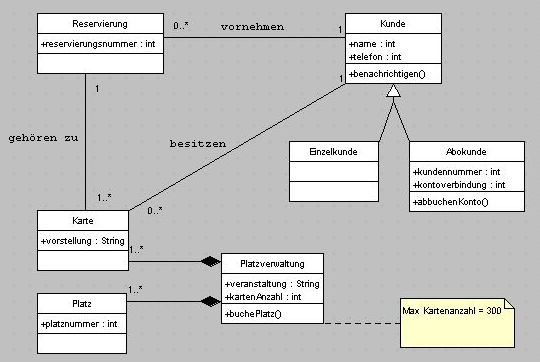
\includegraphics[width=0.8\textwidth]{./inf/SEKII/15_UML_Klassendiagramme/Aufgabe1.png}
%\end{center}

\subsection{Aufgabe 2: Assoziationen}

Zeichne die Assoziationen zwischen folgenden Klassen (Attribute und Methoden brauchen nicht angegeben
werden):

\begin{compactenum}[a)]
\item Ampel, Lampe
\item Baum, Birke, Buche
\item Auto, Mensch, Reifen, Lenkrad, BMW
\item Tisch, Stuhl, Tafel, Raum
\item Schule, Schüler, Lehrer, Klassenraum, Direktor (ein Direktor ist der
Lehrer, der die Schule leitet) 
\end{compactenum}


\subsection{Aufgabe 3: Bestandteile eines Computers}

Beschreibe in einem Klassendiagramm den Aufbau eines Computers. Die
nachfolgende Abbildung soll dafür als Gedächtnisstütze dienen.

\begin{center}
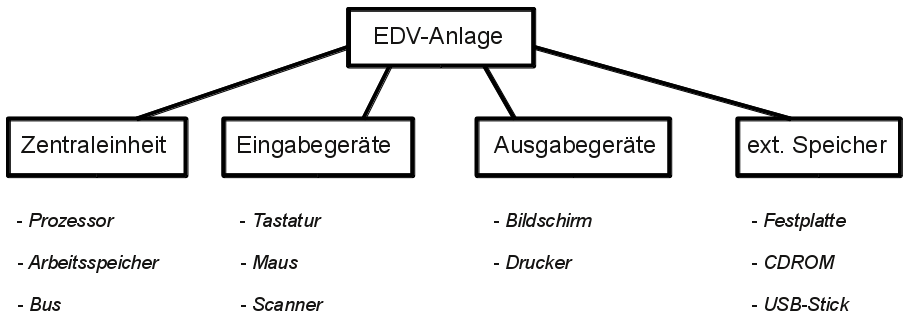
\includegraphics[width=0.7\textwidth]{./inf/SEKII/15_UML_Klassendiagramme/Computer-Komponenten.png}
\end{center}


\subsection{Aufgabe 4: Möbelfirma}

Es soll ein EDV-System für eine Möbelfirma entwickelt werden. Das EDV-System
soll sowohl die Kunden wie auch die zur Verfügung stehenden Artikel verwalten.

\begin{compactenum}[a)]
\item Ein Mitarbeiter der Möbelfirma gibt die nachfolgende Erklärung zu den
 Anforderungen an das benötigte EDV-System:

\begin{quotation}
\noindent Jeder Artikel wird durch seine Artikelnummer gekennzeichnet.
Das EDV-System muss abspeichern, wie viele Stücke eines Artikels zur Zeit im
Lager verfügbar sind. Kunden können einen oder mehrere Artikel (in beliebiger
Stückzahl) bestellen. Wenn der Artikel nicht im Lager vorhanden ist, wird er
bei einem Lieferanten bestellt. Damit dies automatisch geschehen kann, muss das
EDV-System abspeichern, welcher Artikel von welchem Lieferanten geliefert wird.
Jeder Artikel wird von nur einem Lieferanten geliefert. Von den Lieferanten
müssen Firmenname, Adresse und Telefonnummer bekannt sein. Zur Bestellung von
Artikeln muss das System automatisch ein Fax an einen Lieferanten schicken
können. Von den Kunden werden der Name, die Adresse und die Telefonnummer
abgespeichert. Zu Werbezwecken muss automatisch ein Brief an einen Kunden
geschrieben werden können.
\end{quotation}

Entwirf ein Klassendiagramm, das die Beschreibung grafisch darstellt. Gehe
dabei in folgenden Teilschritten vor:

\begin{compactenum}[1.]
\item Entscheide, welche Klassen es gibt.
\item Trage die Attribute und die Methoden jeder Klasse ein.
\item Beschreibe die Beziehung zwischen den Klassen.
\end{compactenum}

\item Zu den Artikeln erklärt der Mitarbeiter der Möbelfirma noch weitere
Details.  Erweitere das Klassendiagramm entsprechend:

\begin{quotation}
\noindent Die Artikel werden nach Holzmöbeln und Polstermöbel sortiert. Für
Holzmöbel muss die Holzart abgespeichert werden. Bei Polstermöbeln ist dagegen
zwischen verschiedenen Stoffmustern zu unterscheiden. Zu den Holzmöbeln zählt
z.B. ein Tisch. Für einen Tisch werden die Länge und die Breite abgespeichert.
Ein weiteres Holzmöbelstück ist ein Stuhl. \ldots\ Ein spezielles
Polstermöbelstück ist das Sofa. Für ein Sofa werden die Länge und die Breite
angegeben. \ldots
\end{quotation}
\end{compactenum}



\subsection{Aufgabe 5: Bank} 

Es soll ein EDV-System für eine Bank entwickelt werden. Ein Mitarbeiter der Bank
gibt die nachfolgende Erklärung zu der Verwaltung von Konten für die Kunden der
Bank. Identifiziere anhand der Beschreibung Klassen, Attribute, Methoden,
Assoziationen und Vererbungshierarchien und zeichne sie in ein Klassendiagramm
ein:

\begin{quotation}
\noindent Eine Person wird Kunde, wenn sie ein Konto eröffnet. Ein Kunde kann
beliebig viele weitere Konten eröffnen. Für jeden neuen Kunden werden dessen
Name, Adresse und das Datum der ersten Kontoeröffnung erfasst. Bei der
Kontoeröffnung muss der Kunde gleich eine erste Einzahlung vornehmen.
Wir unterscheiden Girokonten und Sparkonten. Girokonten dürfen bis zu einem
bestimmten Betrag überzogen werden. Für jedes Konto wird ein individueller
Habenzins, für Girokonten auch ein individueller Sollzins festgelegt; außerdem
besitzt jedes Konto eine eindeutige Kontonummer. Für jedes Sparkonto wird die
Art des Sparens - z.B. Festgeld - gespeichert. Ein Kunde kann Beträge einzahlen
und abheben. Des weiteren werden Zinsen gutgeschrieben und bei Girokonten
Überziehungszinsen abgebucht. Um die Zinsen zu berechnen, muss für jede
Kontobewegung das Datum und der Betrag notiert werden. Die Gutschrift/Abbuchung
der Zinsen erfolgt bei Sparkonten jährlich und bei den Girokonten
quartalsweise. Ein Kunde kann jedes seiner Konten wieder auflösen. Bei der
Auflösung des letzten Kontos hört er auf, Kunde zu sein.
\end{quotation}


\subsection{Aufgabe 6: Werkstatt}

Es soll ein EDV-System für eine Werkstatt entwickelt werden. Das EDV-System
soll sowohl die Kunden wie auch die in Reparatur gegebenen Fahrzeuge verwalten.
Entwirf ein Klassendiagramm, das die nachfolgende Beschreibung grafisch
darstellt:

\begin{quotation}
\noindent Eine Person wird Kunde, wenn sie zum ersten Mal ein Fahrzeug zur
Reparatur bringt. Ein Kunde kann beliebig viele Fahrzeuge zur Reparatur
bringen. Für jeden neuen Kunden werden dessen Name, Adresse und das Datum der
ersten Reparatur erfasst.

Wir unterscheiden bei den Mitarbeitern zwischen Meister, Büroangestellten und
Mechanikern und bei den Fahrzeugen zwischen Autos und Motorrädern. Für jedes
Fahrzeug wird die Marke, die Farbe und das Kennzeichen gespeichert. Für Autos
wird zusätzlich auch die Anzahl der Türen festgehalten. Kunden, die Fahrzeuge
zur Reparatur bringen, bekommen standardmäßig ein halbes Jahr Garantie, sie
können sich aber auch eine längere Garantiezeit kaufen. Für die Reparatur muss
ein Termin vereinbart werden. Die Reparaturkosten variieren, während die
Garantiekosten gestaffelt sind.
\end{quotation}
